\chapter{AI in Image Compression}
\label{ch:ai-image-compression}

In this chapter I will breifly summarise my works till March 17, 2020. The full version of this report can be found here: 
\href{https://github.com/KishoreKaushal/btp-report-phase2/blob/master/btp_report.pdf}{midsem-report.pdf}

\section{Image processing and key phases}

Image processing is manipulating an image in order to enhance it or extract information from it. 
It is widely useed in medical visualization, biometrics, self-driving vehicles, gaming, surveillance, and law enforcement. It can used in various ways: visualization, restoration, imformation retrieval, pattern recognition, etc.

\vspace{1em}
\begin{figure}[!ht]
    \label{fig:keyPhasesOfImageProcessing}
    \centering
    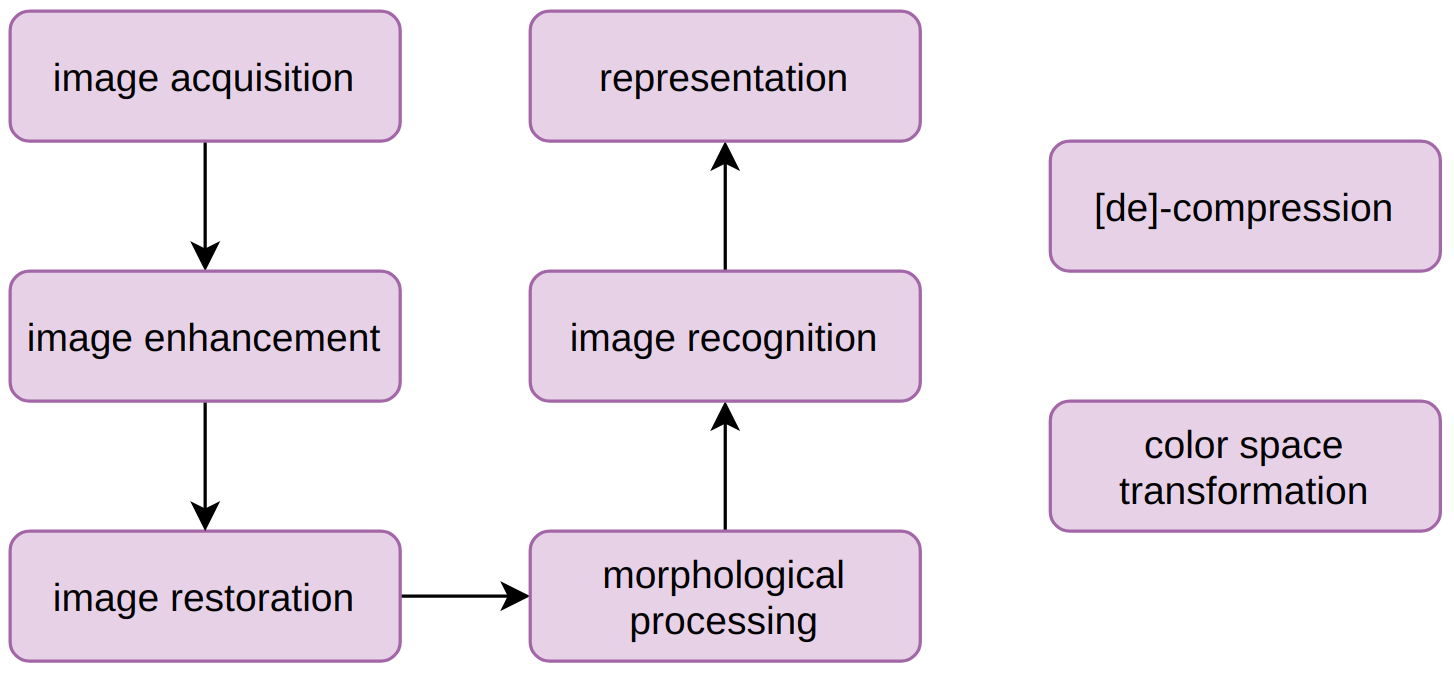
\includegraphics[width=0.60\textwidth]{../fig/midsemwork/keyPhasesOfImageProcessing.png}
    \caption{Steps for dimensionality reduction using PCA}
\end{figure}

\pagebreak
General approach of image processing involves eight key phases: image acquisition, image enhancement, image restoration, color space transformation, compression or decompression, morphological processing, recognition, and representation. 
It is very difficult to carry out these steps manually on a very big data, this is where AI and ML algorithms become very helpful.



\section{Compression}

A data compression algorithm transforms the data to occupy a less space.
The original data is encoded by a program called encoder, to a compressed  representation using a fewer number of bits.
Decoder is responsible for decompressing the compressed representation.

There are two kinds of compression technique: lossy compression and lossless compression. 
The compression technique where the decompressed data is exactly same as original data is called as lossless compression otherwise it is known as lossy compression technique because some information is lost during coding-encoding phase.

Two well-known codecs for image compression are JPEG and PNG. PNG is lossless and JPEG is lossy.

\section{Compression using PCA}

Principal components analysis (PCA) is one of a family of techniques for taking high-dimensional data, and using the dependencies between the variables to represent it in a more tractable, lower-dimensional form, without losing too much information. 
PCA is one of the simplest and most robust ways of doing such dimensionality reduction.
PCA is mathematically defined as an orthogonal linear transformation that transforms the data to a new coordinate system such that the greatest variance by some scalar projection of the data comes to lie on the first coordinate (called the first principal component), the second greatest variance on the second coordinate, and so on.


Let $W$ be a $d \times d$ matrix whose columns are the principal components of $X$. The transformation $T = X W$ maps a data vector $x_{(i)}$ from an original space of $d$ variables to a new space of $d$ variables which are uncorrelated over the dataset. However, not all the principal components need to be kept. Keeping only the first $L$ principal components, produced by using only the first $L$ eigenvectors, gives the truncated transformation:

$T_L = XW_L$


where the matrix $T_L$ now has $n$ rows but only $L$ columns. In other words, PCA learns a linear transformation 
$t = W^{T}x, x \in \Re^{d}, t \in \Re^{L}$, where the columns of $d \times L$ matrix $W$ form an orthogonal basis for the $L$ features (the components of representation t) that are decorrelated. By construction, of all the transformed data matrices with only $L$ columns, this score matrix maximises the variance in the original data that has been preserved, while minimising the total squared reconstruction error $\left \| TW^T - T_LW_L^T\right \|_2^2 or \left \| X - X_L \right \|_2^2$.

The basic steps for computing the PCA is as follows:

\begin{enumerate}
    \item Standardize the d-dimensional dataset.
    \item Construct the covariance matrix.
    \item Decompose the covariance matrix into its eigenvectors and eigenvalues.
    \item Sort the eigenvalues by decreasing order to rank the corresponding eigenvectors.
    \item Select $L$ eigenvectors which correspond to the $L$ largest eigenvalues, where $L$ is the dimensionality of the new feature subspace $L \leq d$.
    \item Construct a projection matrix $W_L$ from the "top" $L$ eigenvectors.
    \item Transform the $d$-dimensional input dataset $X$ using the projection matrix $W_L$ to obtain the new $L$-dimensional feature subspace.
\end{enumerate}

\vspace{1em}

\begin{figure}[!ht]
    \label{fig:dimensionalityReductionSteps}
    \centering
    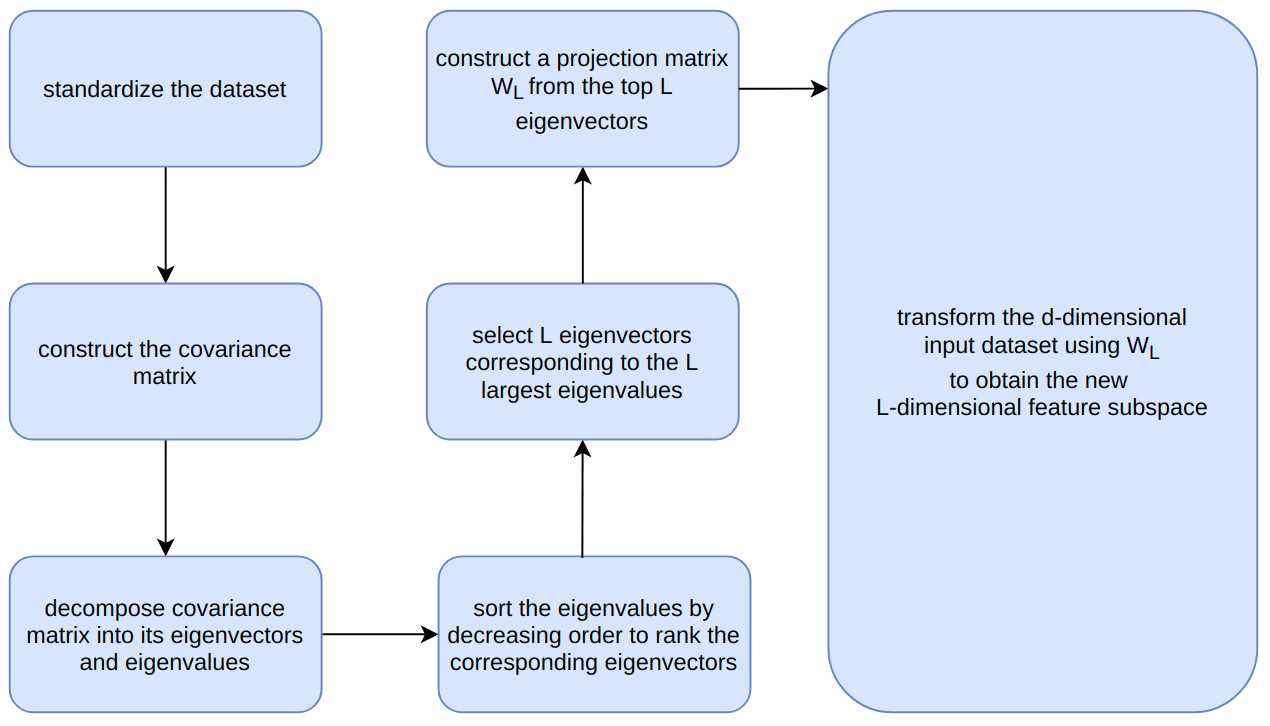
\includegraphics[width=0.75\textwidth]{../fig/midsemwork/dimensionalityReductionUsingPCA.png}
    \caption{Steps for dimensionality reduction using PCA}
\end{figure}


\section{Image compression using PCA}


We will follow the steps mentioned in the previous section for dimensionality reduction using PCA. The results of the experiments are shown in the figure 5.2.

\begin{figure}[!ht]
    \label{fig:imageCompressionUsingPCA}
    \centering
    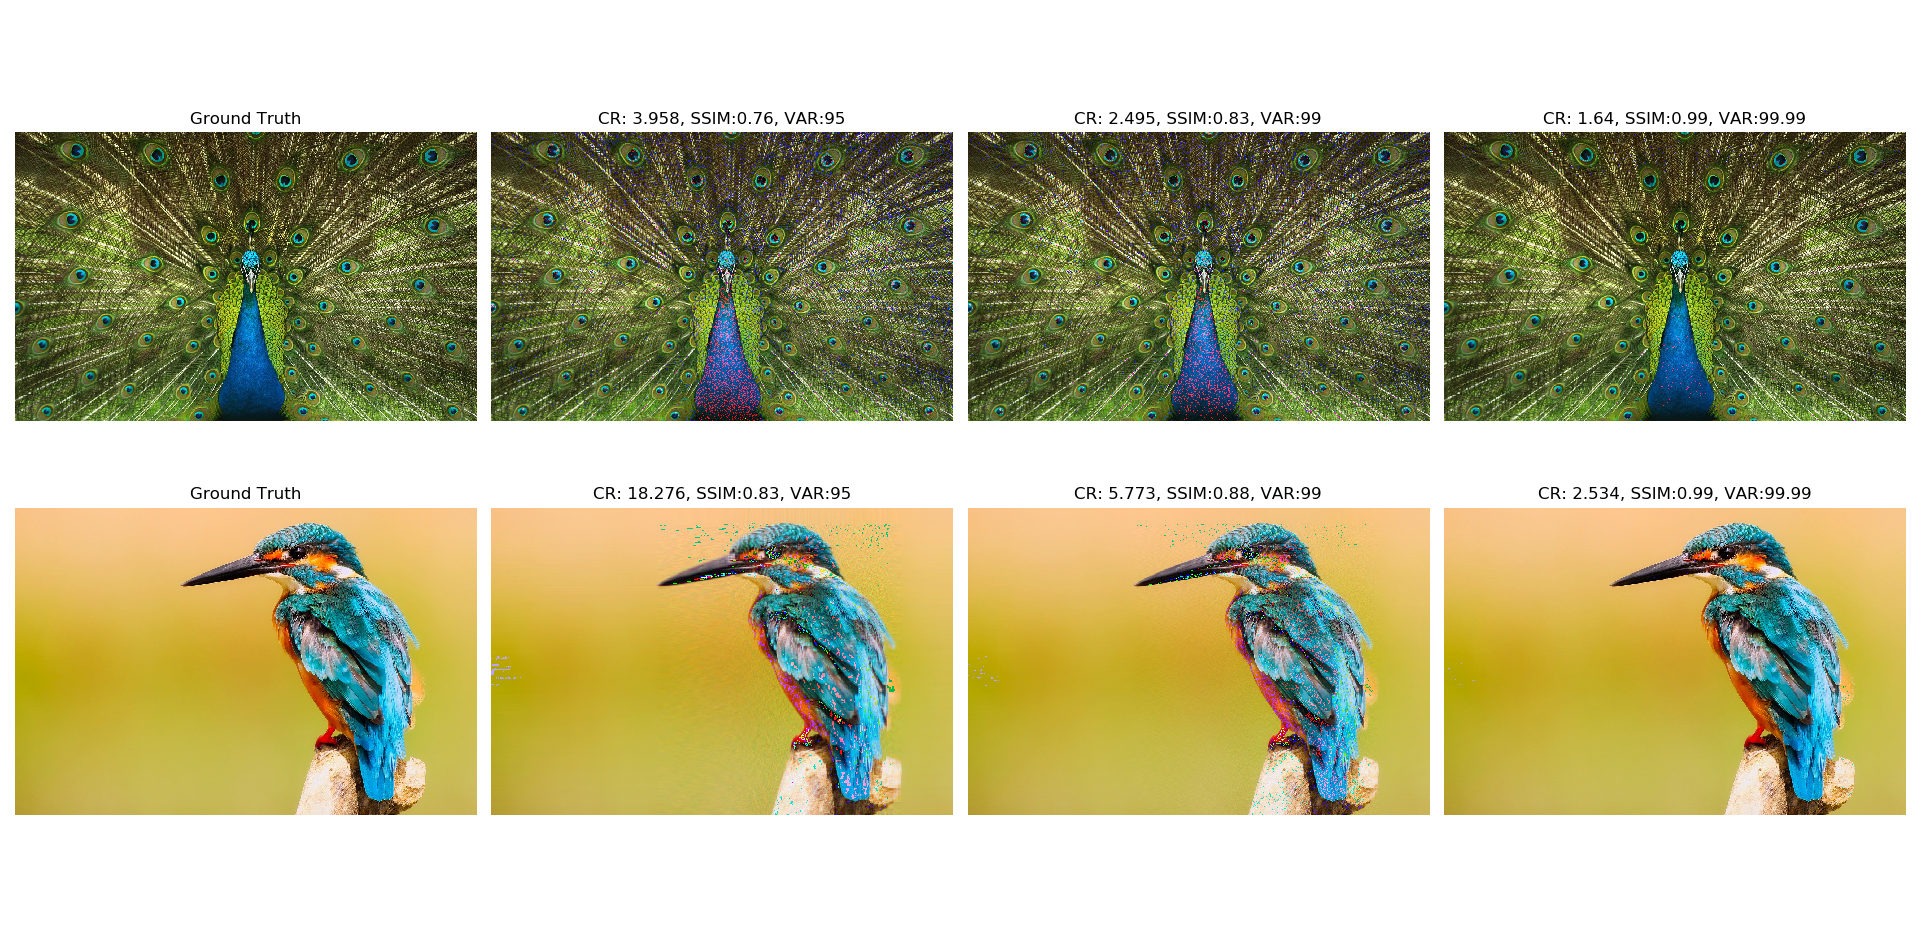
\includegraphics[width=1\textwidth]{../fig/midsemwork/ImageCompressionWithPCA.png}
    \caption{CR = Compression Ratio, SSIM = Structural Similarity Index, VAR = Variance. Results of compression using the PCA method. Higher variance leads to more number of principal components and higher is the reconstructed image quality and lower the compression rate.}
    
\end{figure}

You can find the implementation of the image compression using PCA here:

\href{https://github.com/KishoreKaushal/ImageCompression/tree/master/PCA}{@KishoreKaushal/ImageCompression/}

It is clear from this experiment that higher variance leads to more number of principal components and higher is the reconstructed image quality and lower the compression rate. Infact, the first $L$ principal components is selected to get atleast the given number of variance.

\section{JPEG Compression}

I will summarise the JPEG compression algorithm using the flowchart shown in the next figure.
You can refer to my \href{https://github.com/KishoreKaushal/btp-report-phase2/blob/master/btp_report.pdf}{previous report} for a detailed analysis.

The image is first split in $8x8$ blocks. 
Then, the image in RGB space is transformed to YCbCr space, followed by a downsampling and a forward discrete cosine transform (DCT). 
The final blocks are then quantized with an quantization matrix which is adjusted accoirding to the quality factor. 
Finally, the quantized block of values are arranged in form of a row-vector and entropy encoded.

\begin{figure}[!ht]
    \centering
    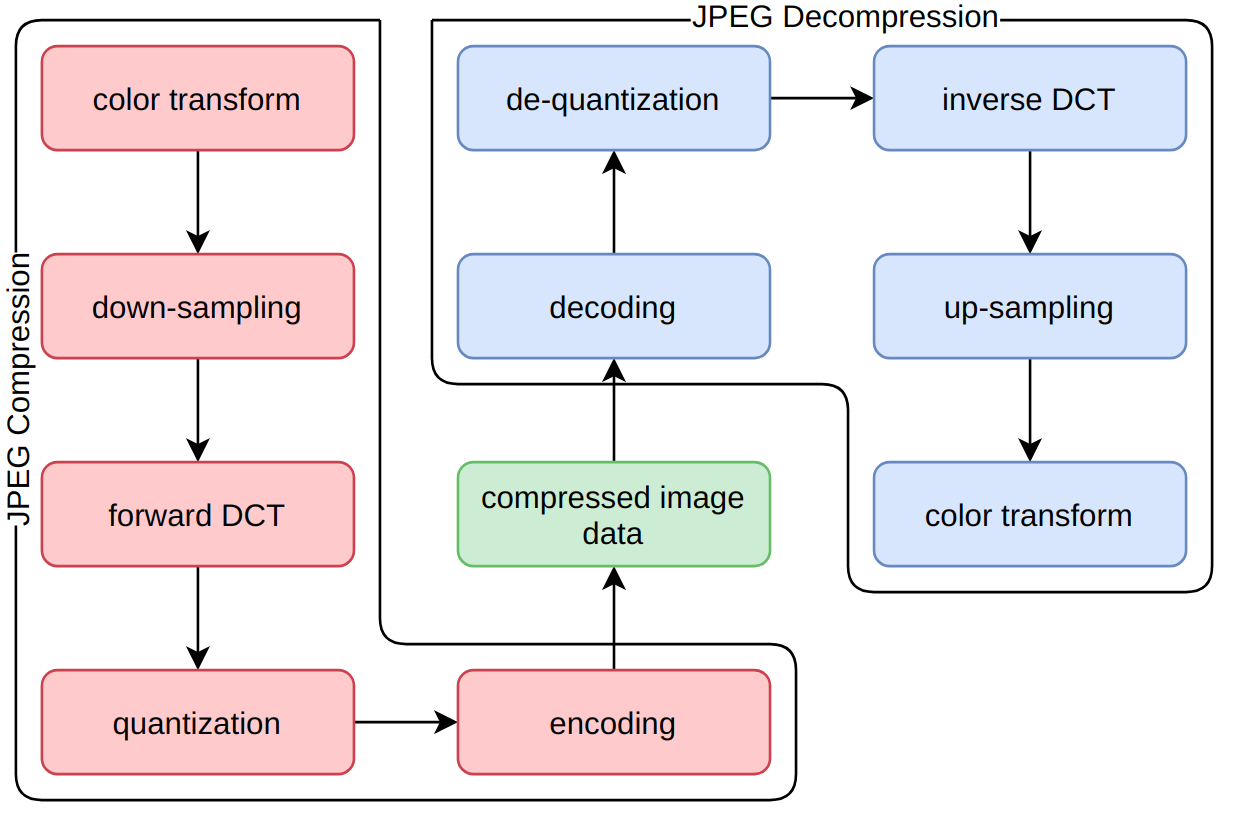
\includegraphics[width=0.80\textwidth]{../fig/midsemwork/jpeg-codec.png}
    \caption{JPEG Schematic}
    \label{fig:jpegSchematic}
\end{figure}


\section{Perceptual Image Comparison}

Prakash et al. \cite{Prakash2017} introduced a powerful CNN tailored to the specific task of semantic image understanding to achieve higher visual quality in lossy compression. 
A modest increase in complexity is incorporated into the encoder which allows a standard, off-the-shelf jpeg decoder to be used. 
While JPEG encoding may be optimized for generic images, the process is ultimately unaware of the specific content of the image to be compressed. 
This technique makes JPEG content-aware by designing and training a model to identify multiple semantic regions in a given image.


The idea here is to locate multiple regions of interest (ROI) within a single image and noting the fact that it's not an object detection problem and hence the precision of the boundary doesn't matter. 
Also, the model needs to learn a single class-invariant feature map by learning separate feature maps for each of a set of object classes and then summing over the top features.

We then discussed methods for object localization like multi-structure region of interest and CAM which allow us to detect the region of interest in the image.
We can then use this to train our omodel to generate a better quantization matrix for a particular task.


\section{Conclusion}

In this chapter we breifly discussed our works before till Mar 17, 2020. In the next phase we will discuss our works on after Mar 17, 2020.